\documentclass[xcolor=svgnames, usepdftitle=false, aspectratio=169]{beamer}
\usepackage{pgfpages}
\setbeameroption{hide notes}
\usepackage[theorems]{tcolorbox}

\frenchspacing

% --- THEME ---
\usetheme[progressbar=frametitle]{metropolis}

\useoutertheme{metropolis}
\useinnertheme{metropolis}
\usefonttheme{metropolis}
\usecolortheme{dove}  % spruce, metropolis, dove, crane, beaver, seagull
\setbeamercolor{background canvas}{bg=transparent}
\usecolortheme[named=DarkOrange]{structure}
\usefonttheme[onlymath]{serif}

% \setbeamersize{text margin left=5.03cm}
\setbeamercolor{title separator}{fg=DarkOrange}

% --- HACKS ---
% Hide numbers on standout slides.
\setbeamertemplate{frame numbering}{
    \ifbool{metropolis@standout}{}{
        \insertframenumber
    }
}
\setbeamertemplate{frame numbering}[counter]  % none, counter, fraction

% Avoid font-warning with itemize bullets.
\renewcommand\textbullet{\ensuremath{\bullet}}

% --- PACKAGES ---
\usepackage[UKenglish]{babel}
\usepackage[utf8]{inputenc}
\usepackage{lmodern}
\usepackage[T1]{fontenc}

% \usepackage{appendixnumberbeamer}
\usepackage{upquote}
\usepackage[straightquotes]{newtxtt}
\usetikzlibrary{positioning}
% \usepackage{minted}
\usepackage{multicol}
\usepackage{xspace}
\usepackage{booktabs}
\usepackage{siunitx}

% --- SETTINGS ---
\graphicspath{{../figures/}}
\setlength{\fboxsep}{0pt}

% --- OWN COMMANDS ---
\newcommand{\bdra}{\ensuremath{\boldsymbol \Rightarrow }~}
\newcommand{\bdla}{\ensuremath{\boldsymbol \Leftarrow }~}
\newcommand{\dra}{\ensuremath{\Rightarrow }~}
\newcommand{\dla}{\ensuremath{\Leftarrow }~}
\newcommand{\mr}[1]{\mathrm{#1}}
\newcommand{\emg}[2]{\texttt{emg#1#2}\xspace}
\newcommand{\empymod}{\texttt{empymod}\xspace}
\newcommand{\ohmm}{\ensuremath{\Omega\,}\text{m}\xspace}
\newcommand{\rmk}[1]{{\color{red}\bfseries #1}}
\newcommand{\maybe}[1]{{\color{gray} #1}}
\newcommand{\todo}{{\color{red}\texttt{TODO:}}\xspace}
\newcommand{\bm}[1]{{\mathbf{#1}}}

% Add page number to slides
\newcommand{\ato}{\addtocounter{framenumber}{1}}

% --- TITLE-STUFF ---

\newcommand{\ttitle}{Time-domain CSEM modelling}
\title{\vspace{2.5cm}\color{white}{\ttitle}}
\subtitle{\color{white}{using frequency- and Laplace-domain computations}}
\date{\color{white}{20 October 2021}}
\author{\vspace{-.3cm}\color{white}{Dieter Werthmüller and Evert Slob, TU Delft}}
\institute{}

\hypersetup{pdftitle={\ttitle}, allcolors=NavyBlue, colorlinks=true}

% --- SLIDES ---
\begin{document}
\metroset{block=fill}  % Fills the block-environment
\usebackgroundtemplate{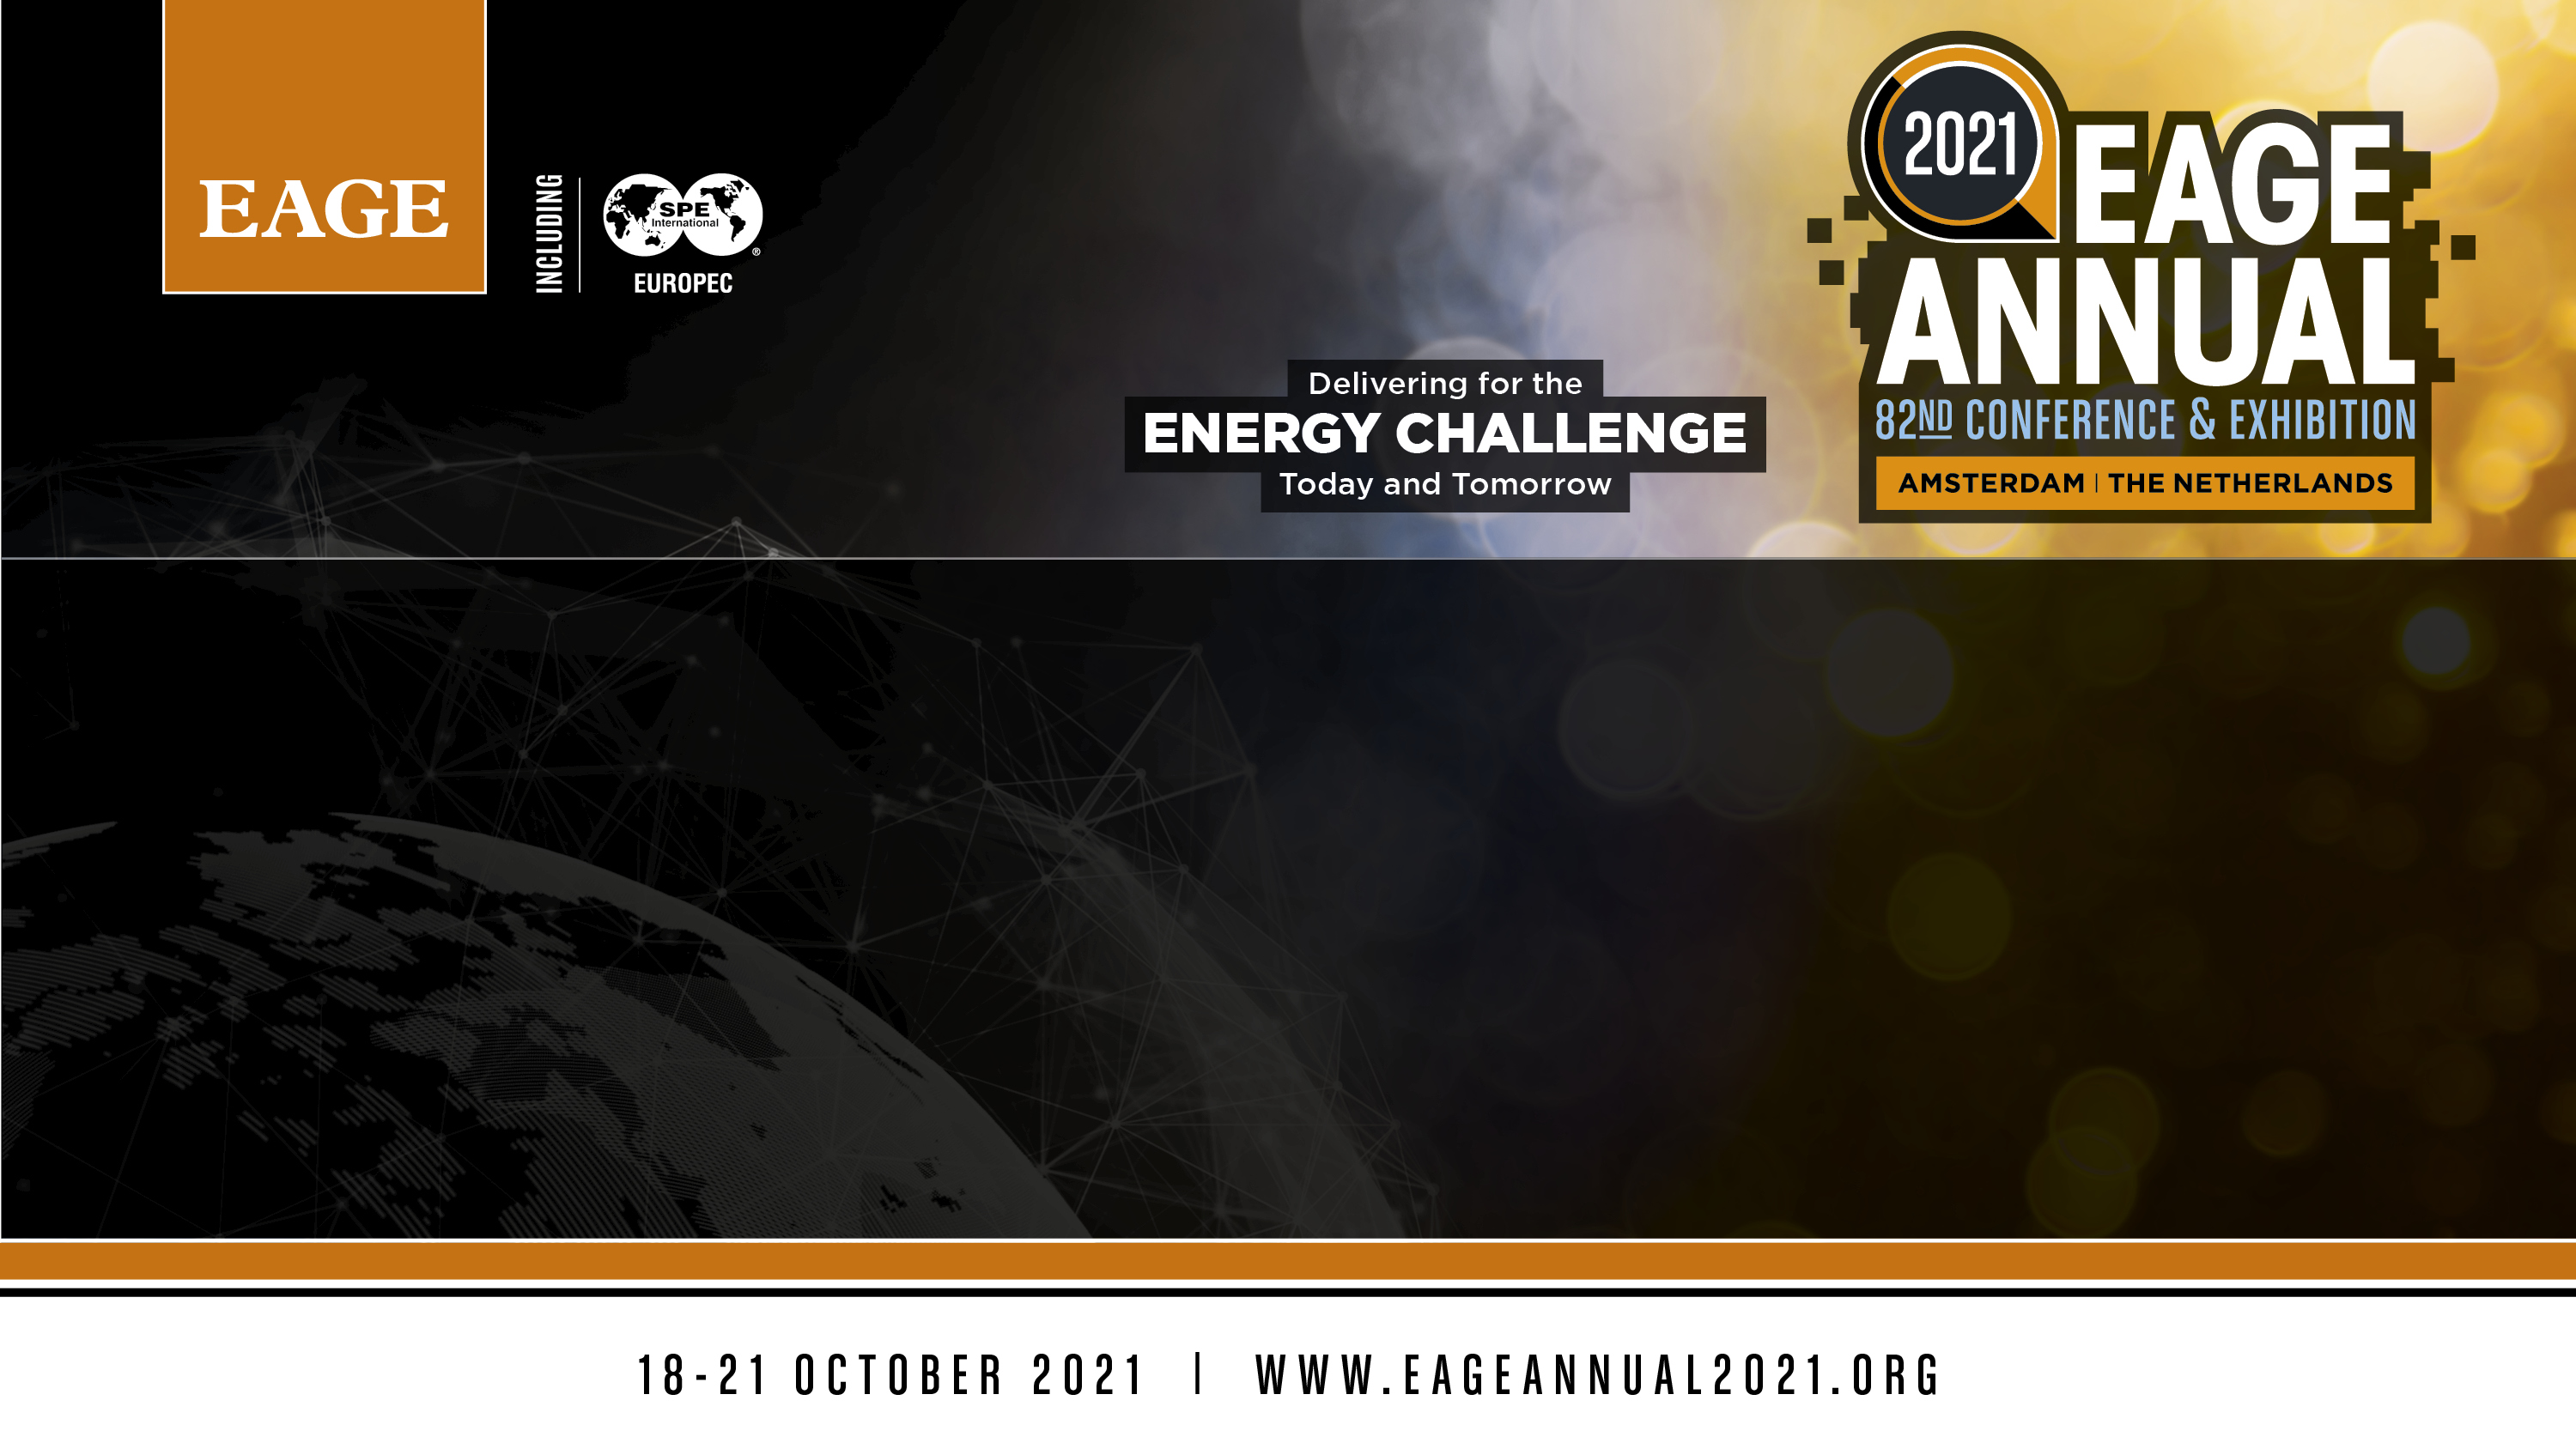
\includegraphics[width=\paperwidth]{SlideTitle}}

\ato
\maketitle % ---------------------------------------------------------------- %
\usebackgroundtemplate{
\includegraphics[width=\paperwidth]{SlideContent}}

\ato
\section{Part I: frequency to time} % --------------------------------------- %

\begin{frame}
  {Fast Fourier transform of EM data for computationally expensive kernels
  $^\dagger$}

  \begin{columns}[t]
    \column{.33\textwidth}

    \begin{block}
      {Solver}
      \begin{itemize}
        \item Fast
        \item Robust over wide range of frequencies
      \end{itemize}
    \end{block}

    \column{.33\textwidth}

    \begin{block}
      {Gridding}

      \begin{itemize}
        \item Adaptive
        \item $f$-dependent
      \end{itemize}
    \end{block}

    \column{.33\textwidth}

    \begin{block}
      {Transform}
      As few frequencies as possible
      \begin{itemize}
        \item Log-scale\\(DLF; FFTLog)
        \item Interpolation
        \item Zero-padding
      \end{itemize}
    \end{block}

  \end{columns}

  \vspace{-1cm}
  \alert{Conclusions}
  \begin{itemize}
    \item 15--25 frequencies are usually enough
    \item Equally applies for $t\rightarrow f$
  \end{itemize}

  \vspace{.5cm}
  \footnotesize
  $^\dagger$ Werthmüller, Mulder, and Slob, 2021, GJI, 10.1093/gji/ggab171.

\end{frame}

\begin{frame}
  {Example using FFTLog and Digital Linear Filters}
  \centering

  \only<1>{
    ~\hspace{-1cm}
    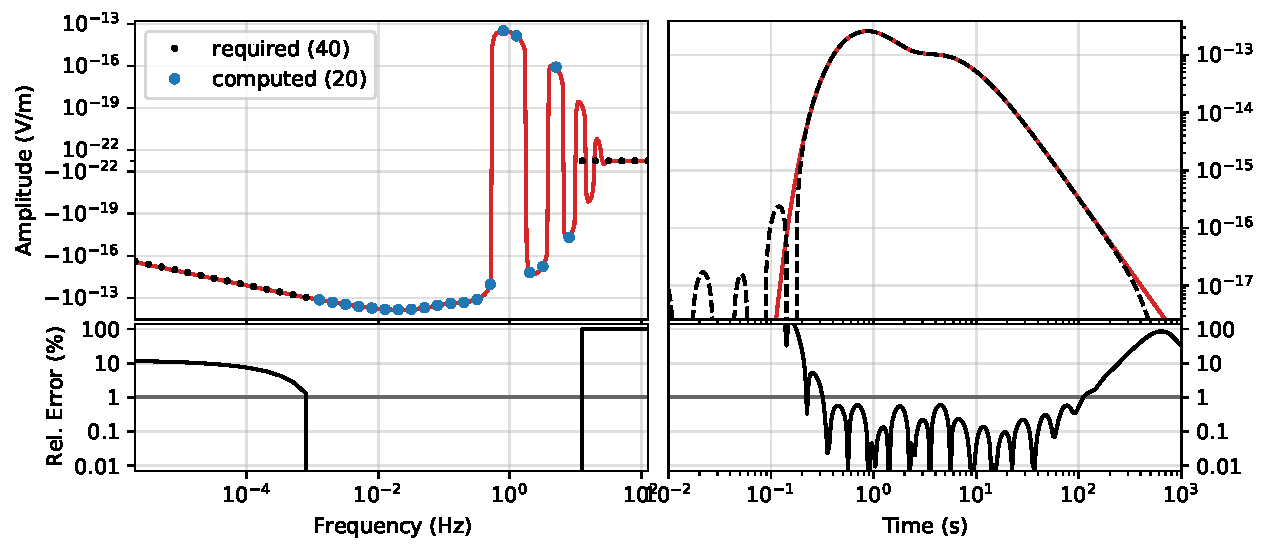
\includegraphics[trim=0 0 290 0, clip, width=.39\textwidth]{01-FFTLog-log}%
    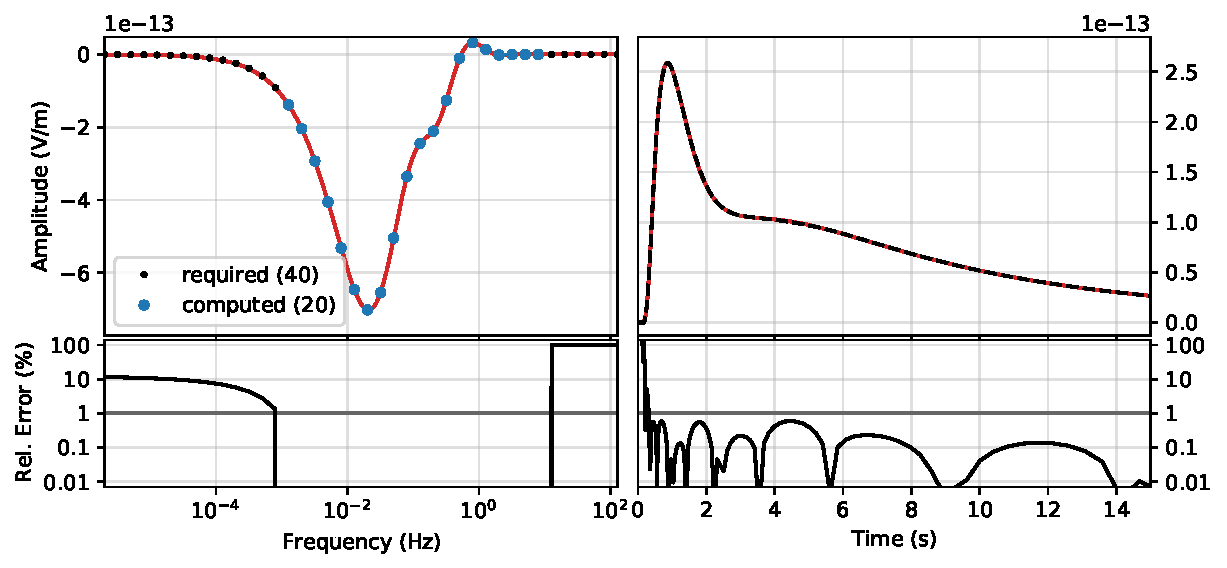
\includegraphics[width=.72\textwidth]{02a-FFTLog-lin}%
  }
  \only<2>{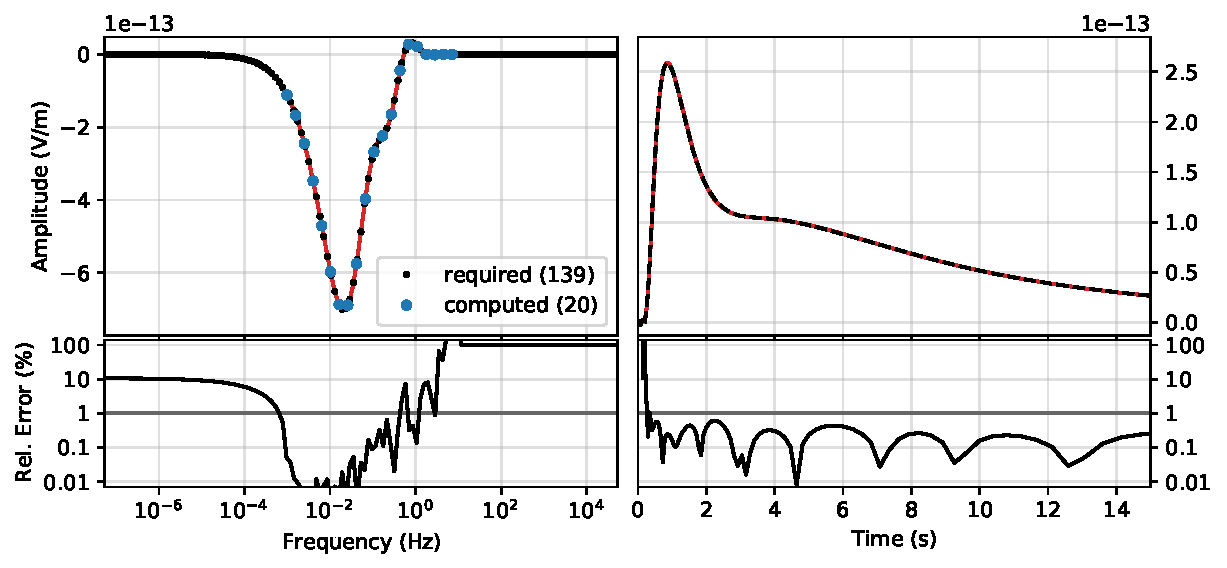
\includegraphics[width=.8\textwidth]{02b-DLF-lin}\ato}
  \only<3>{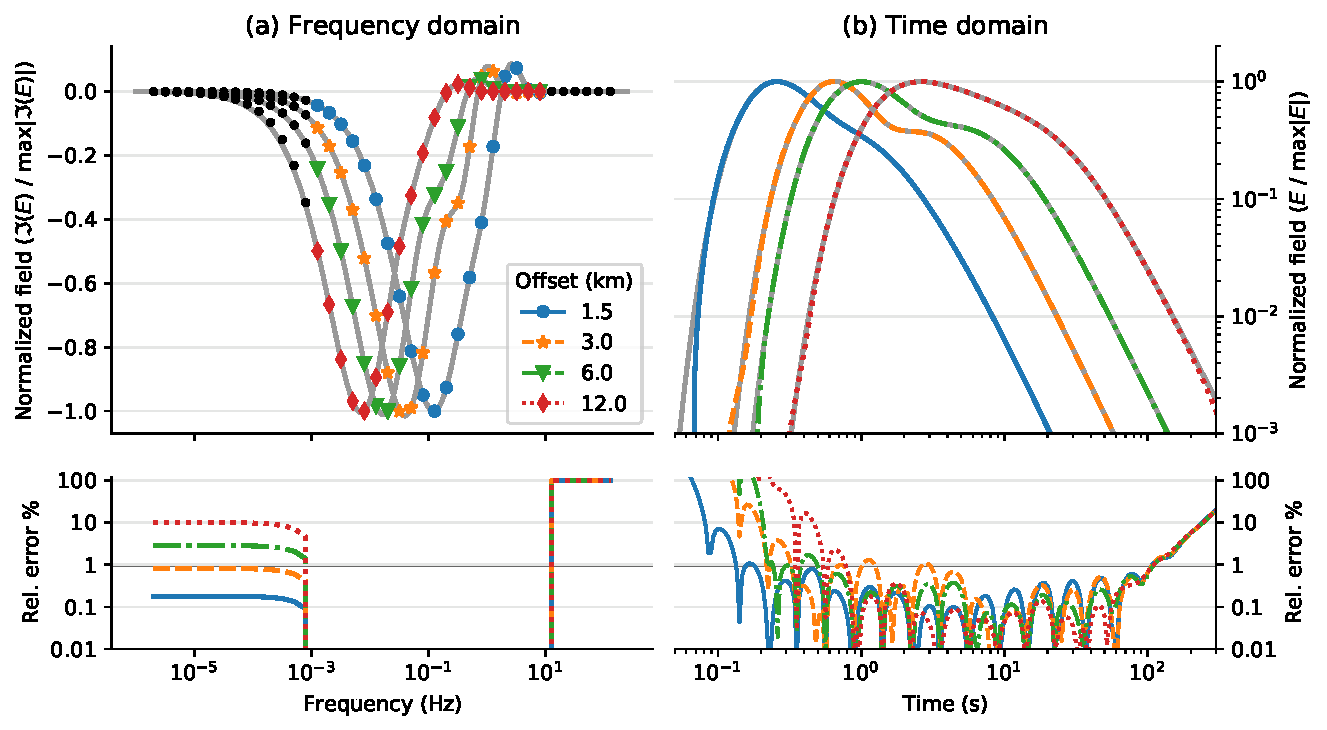
\includegraphics[width=.8\textwidth]{03-multi-offset}\ato}

  \only<-2>{
  \textbullet\ $f<f_\mr{min}$: PCHIP \hfill
  \textbullet\ $f_\mr{min}<f<f_\mr{max}$: Cubic spline \hfill
  \textbullet\ $f>f_\mr{max}$: 0
  }

\end{frame}


\begin{frame}
  {Example: Induced Polarization}

  Also works for 3D or any model, as the transform is unaware of the
  complexity.

  \begin{columns}
    \column{.75\textwidth}
      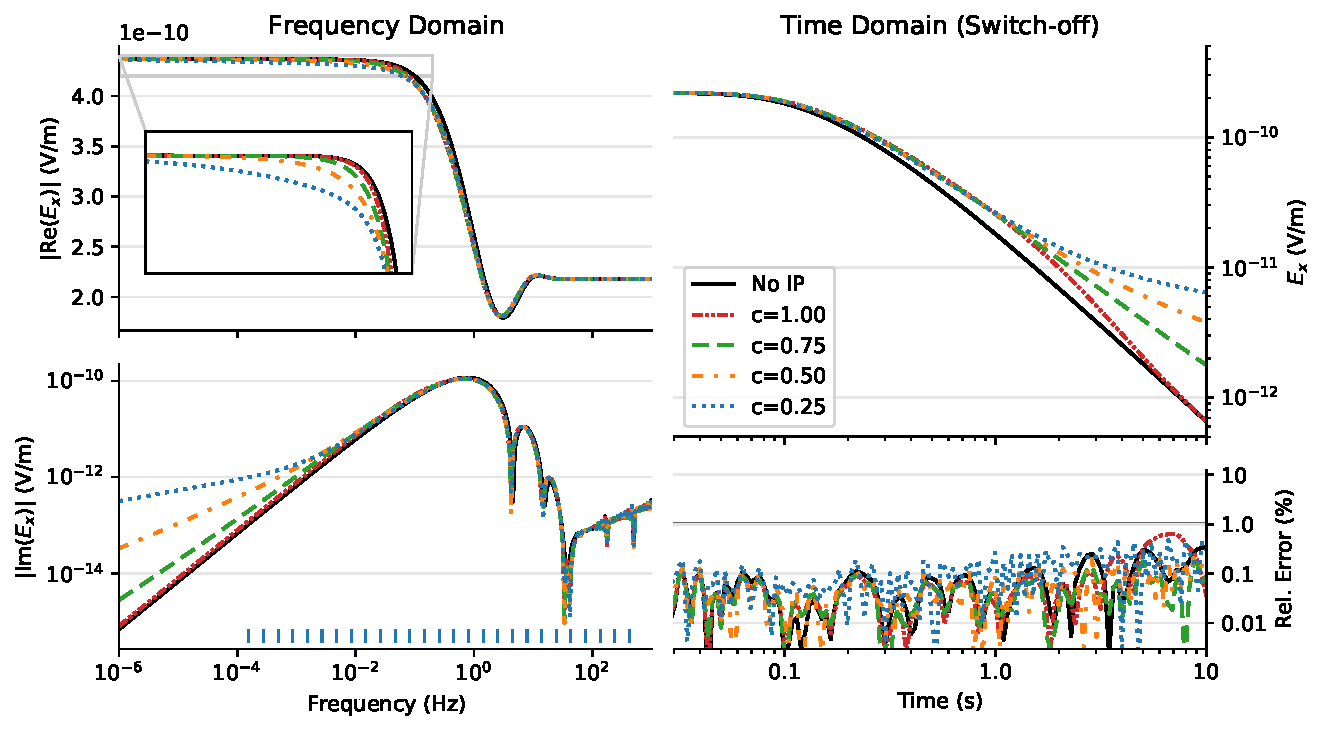
\includegraphics[width=\linewidth]{11-cole-cole-model}
    \column{.25\textwidth}
      %
      \begin{equation}
       ~\hspace{-.5cm} \sigma(\omega) = \sigma_\infty + \frac{\sigma_0 - \sigma_\infty}{1 +
          (\rm{i}\omega\tau)^c}
          \nonumber
      \end{equation}
      %
  \end{columns}

  27 frequencies instead of 747 frequencies (601\,pt filter)

\end{frame}

\ato
\section{Part II: Laplace to time} % ---------------------------------------- %



\begin{frame}  % Motivation
  {Laplace-domain computation: Motivation}
  \centering
  \vspace{-.5cm}

  % Correct for: e^+iwt: + s σ E − ∇ × µ^-1 ∇ × E = − s J
  %              e^-iwt: + s σ E + ∇ × µ^-1 ∇ × E = − s J
  $$
  \tcbhighmath[colframe=SteelBlue]{
    \mr{i}\omega \rightarrow s:
    \qquad
    \textcolor{red}{s} \mu \tilde{\sigma} \mathbf{E} \ +\
    \nabla^2 \mathbf{E} \ =\ -\textcolor{red}{s} \mu \mathbf{J}_\mathrm{s}
  }
  $$

  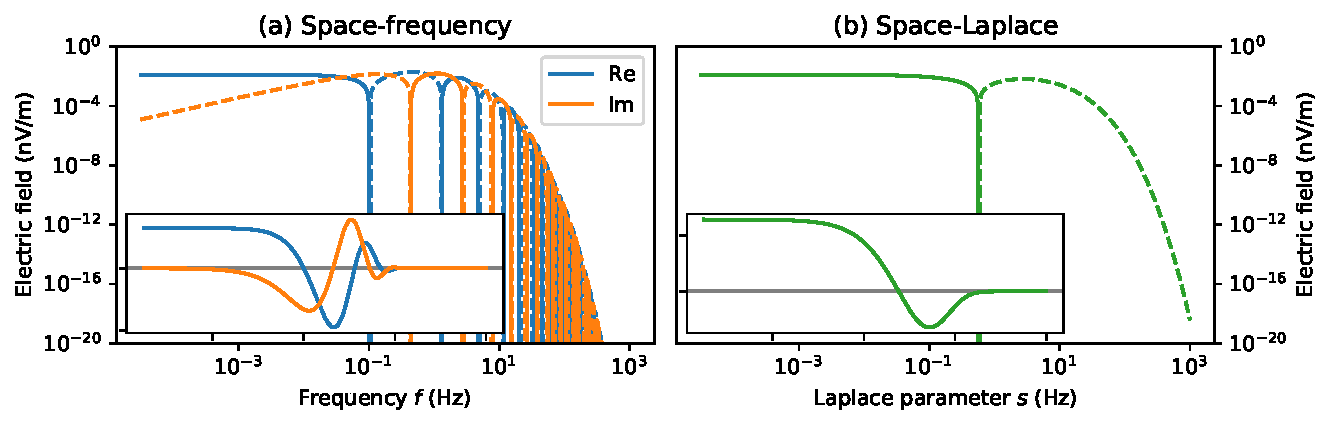
\includegraphics[width=\textwidth]{motivationcomparison}

  \raggedright

  \alert{
    \qquad \bdra \quad  Faster\quad (1) Computation\quad (2) Convergence \quad
    \bdla\\}
  \vspace{.5cm}

\end{frame}

\begin{frame}
  {Computation speed (layered; 3D) \& Convergence (3D)}
  \centering

  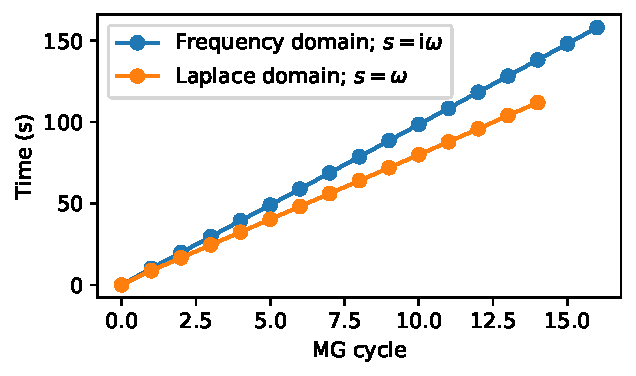
\includegraphics[width=.6\linewidth]{xf-vs-xs}%

  \begin{itemize}
    \item Overall Laplace comp. roughly 2/3 of frequency comp.
  \end{itemize}
\end{frame}

\begin{frame}  % Filter design
  {Digital linear filter for Laplace}

  $$
  F(r) = \int^\infty_0 f(l)K(l r)\mr{d}l \quad \dra \quad
  F(r) \approx \sum^N_{n=1} \frac{f(b_n/r) h_n}{r}
  $$

  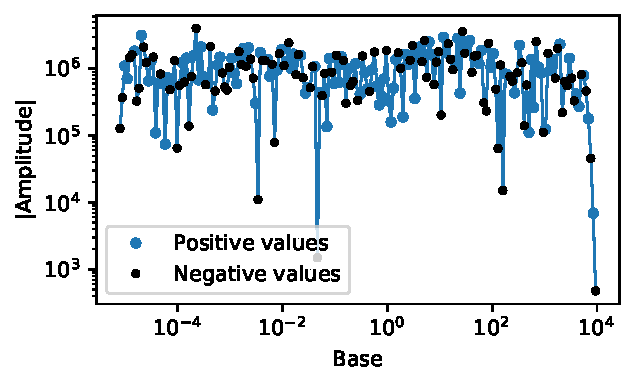
\includegraphics[width=.47\linewidth]{filter-space}\hfill
  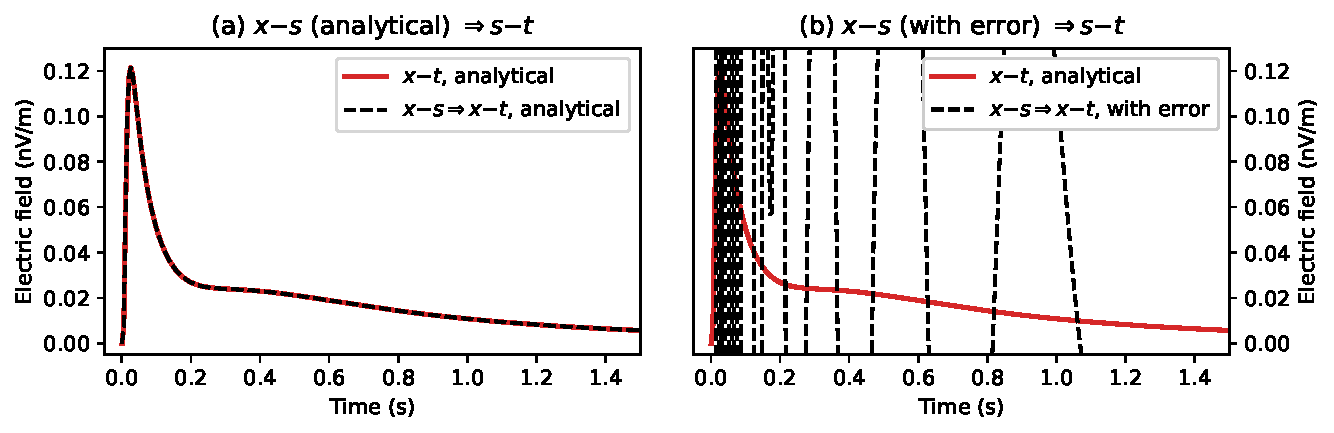
\includegraphics[clip, trim=0 0 320 0, width=.47\linewidth]{s-t_time}%

\end{frame}


\begin{frame}[t]
  {Problem: robustness of the approach}
  ~\vspace{-.8cm}\\
  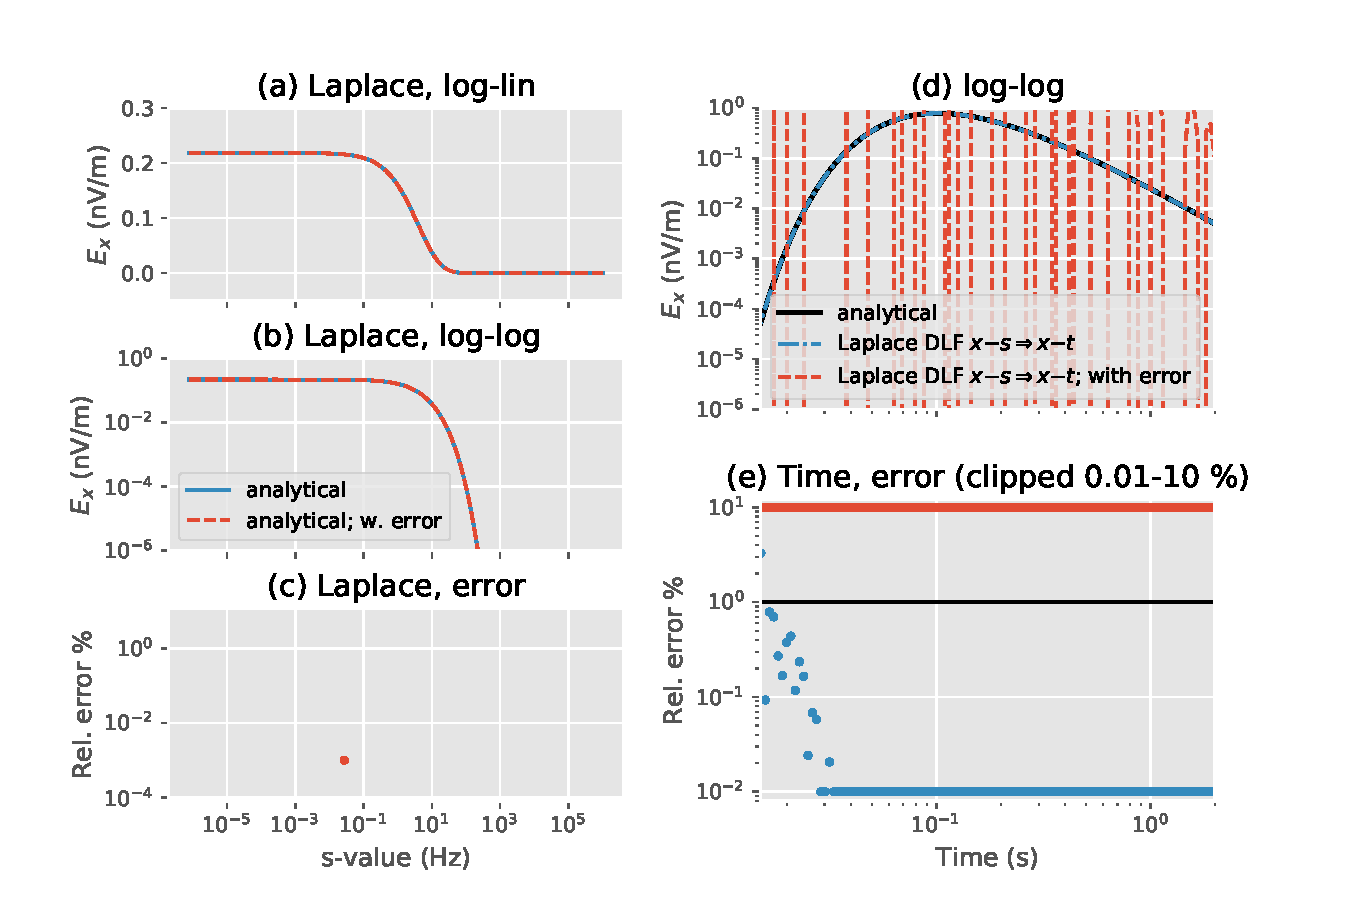
\includegraphics[trim=30 0 40 35, clip, width=.83\linewidth]{s-t_time-2}%

\end{frame}

\ato
\section{Part III: Laplace to frequency} % ---------------------------------- %

\begin{frame}
  {Laplace-to-frequency domain}

  \begin{itemize}\itemsep.5cm
    \item Same motivation as for $s\rightarrow t$: computation speed and
      convergence
    \item Possible to design a linear digital filter
    \item Same limitation as $s\rightarrow t$
    \item Additionally: DLF seems to be offset dependent!
  \end{itemize}

\end{frame}

\ato
\section{Wrap-up} % --------------------------------------------------------- %


\begin{frame}
  {Conclusions}
  \begin{itemize}\itemsep1cm
    \item $f\rightarrow t$: Solver; Method; Gridding;
      \alert{15--25 frequencies are generally enough}
    \item \alert{Laplace: roughly 2/3 computation time} (computation;
      convergence)
    \item $s\rightarrow t$; $s\rightarrow f$: \alert{DLF works; but only for
      very precise results}
  \end{itemize}
\end{frame}

\begin{frame}%
  {References}
  \begin{columns}
    \column{\textwidth}
  \setlength{\columnseprule}{0.4pt}
  % \setlength{\columnsep}{3em}
  \begin{multicols}{2}
  \tiny
  \begin{description}[2cm]
    %
    \item[Ghosh, D. P., 1971,] {\bfseries The application of linear filter
      theory to the direct interpretation of geoelectrical resistivity sounding
      measurements:} Geophysical Prospecting, 19, 192--217;
      \href{https://doi.org/10.1111/j.1365-2478.1971.tb00593.x}{doi:~10.1111/j.1365-2478.1971.tb00593.x}.
    %
    \item[Hamilton, A. J. S., 2000,] {\bfseries Uncorrelated modes of the
      non-linear power spectrum:} Monthly Notices of the Royal Astronomical
      Society, 312, pages 257--284;
      \href{https://doi.org/10.1046/j.1365-8711.2000.03071.x}%
      {doi:~10.1046/j.1365-8711.2000.03071.x}.
    %
    \item[Mulder, W. A., M. Wirianto, and E. Slob, 2008,] {\bfseries
      Time-domain modeling of electromagnetic diffusion with a
      frequency-domain code:} Geophysics, 73, F1--F8;
      \href{https://doi.org/10.1190/1.2799093}{doi:~10.1190/1.2799093}.
    %
    \item[Plessix, R.-E., M. Darnet, and W. A. Mulder, 2007,] {\bfseries An
      approach for 3D multisource, multifrequency CSEM modeling:} Geophysics,
      72, SM177--SM184;
      \href{https://doi.org/10.1190/1.2744234}{doi:~10.1190/1.2744234}.
    %
    \item[Werthmüller, D., 2017,] {\bfseries An open-source full 3D
        electromagnetic modeler for 1D VTI media in Python: empymod:}
        Geophysics, 82(6), WB9--WB19;
        \href{https://doi.org/10.1190/geo2016-0626.1}%
        {doi:~10.1190/geo2016-0626.1}.
    %
    \item[Werthmüller, D., K. Key, and E. C. Slob, 2019,] {\bfseries A tool
        for designing digital filters for the Hankel and Fourier transforms
        in potential, diffusive, and wavefield modeling:} Geophysics, 84(2),
        F47--F56; \href{https://doi.org/10.1190/geo2018-0069.1}%
        {doi:~10.1190/geo2018-0069.1}.
    %
    \item[Werthmüller, D., W. A. Mulder, and E. C. Slob, 2019,] {\bfseries
      emg3d: A multigrid solver for 3D electromagnetic diffusion:} Journal of
      Open Source Software, 4(39), 1463;
      \href{https://doi.org/10.21105/joss.01463}{doi:~10.21105/joss.01463}.
    %
    \item[Werthmüller, D., W. A. Mulder, and E. C. Slob, 2021,] {\bfseries Fast
      Fourier transform of electromagnetic data for computationally expensive
      kernels:} Geophysical Journal International, 226, No. 2, 1336--1347;
      \href{https://doi.org/10.1093/gji/ggab171}{doi:~10.1093/gji/ggab171}.
    %
  \end{description}
\end{multicols}
\end{columns}~\\[.1cm]


Used open-source codes: \empymod (layered models) \& \emg3d (3D models),
\href{https://emsig.xyz}{emsig.xyz}.

Acknowledgment:\\
\scriptsize
This research was conducted within the Gitaro.JIM project funded\\
through MarTERA as part of Horizon 2020 (ERA-NET Cofund).



\end{frame}

\end{document}
